Com o diagrama da arquitectura do sistema, figura~\ref{fig diaact},pretende-se mostrar as várias entidades que podem aceder ao sistema, assim como as várias
actividades que cada uma pode realizar e tarefas para o sistema processar.
Também é realçada a ideia de que alguns dos recursos do sistema só estão dispóniveis ao utilizador depois 
de passar por outros passos, ou seja, o diagrama dá a entender a ordem pelas quais o utilizador e o sistema podem/devem executar as tarefas.\\

\begin{figure}[htbp]
\begin{center}
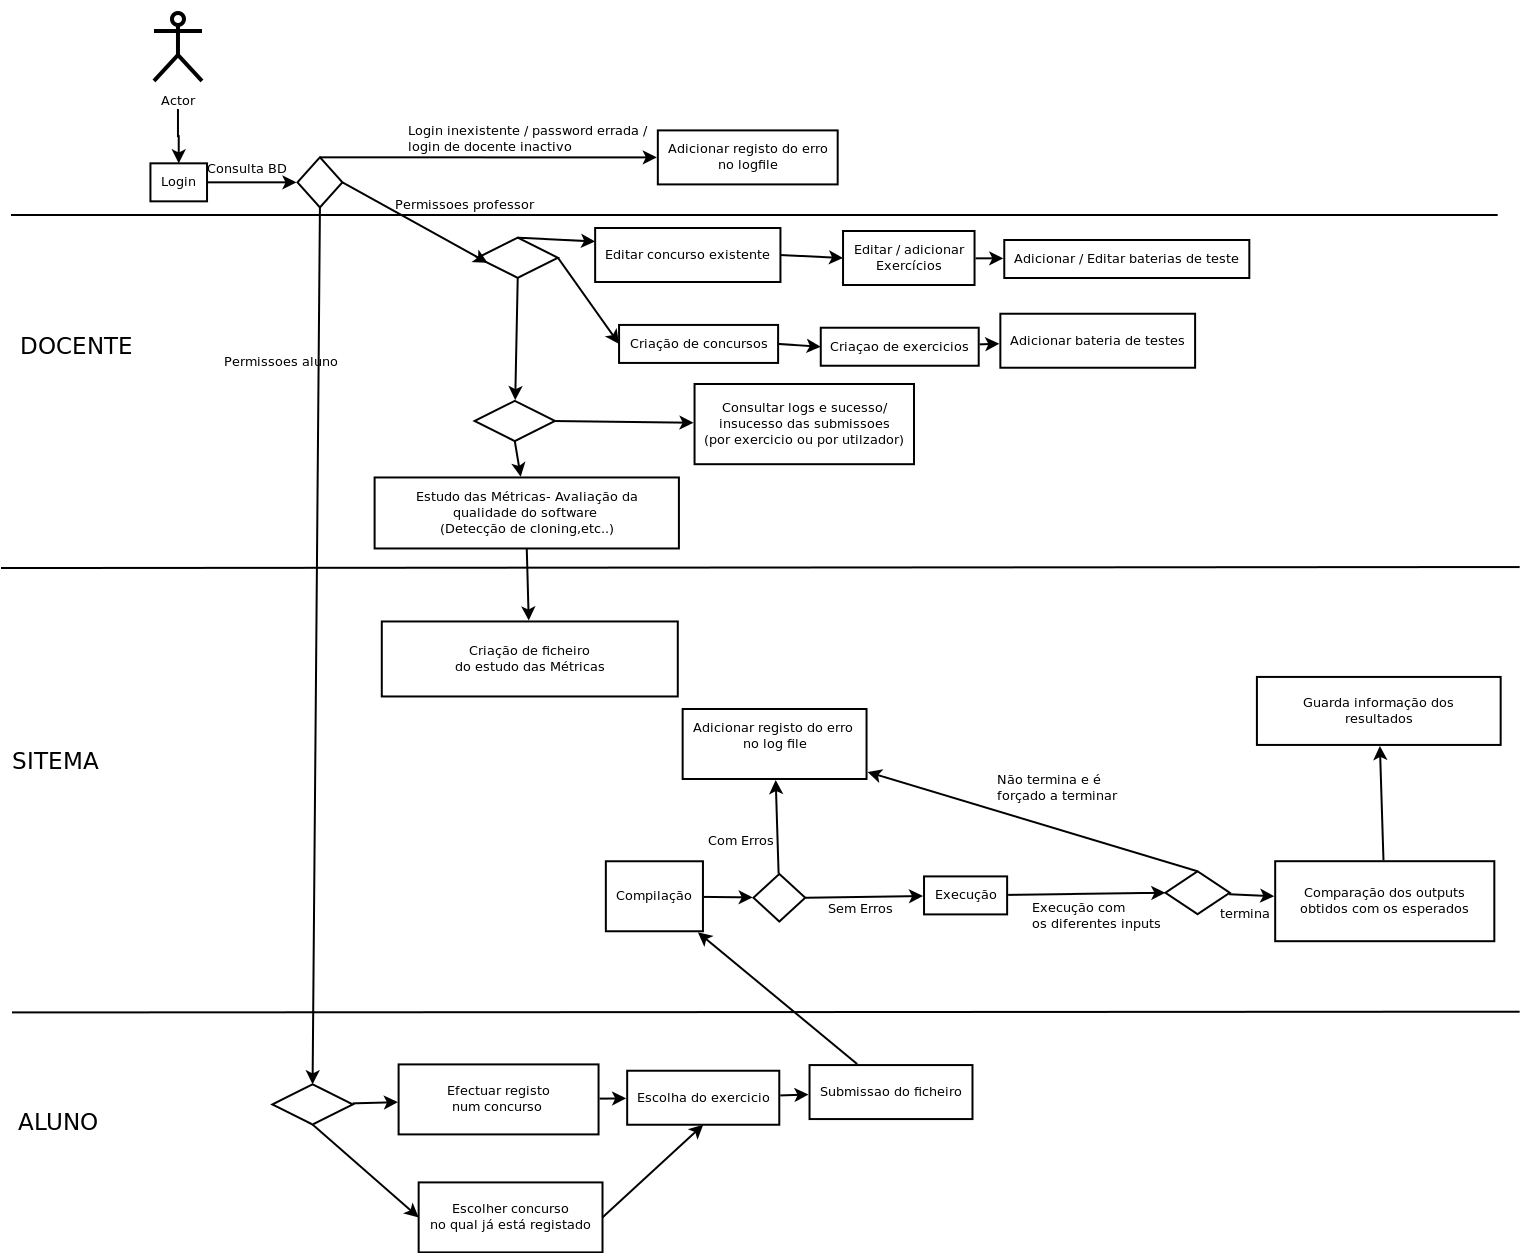
\includegraphics[width=0.5\textwidth]{Images/EL-PI}
\caption{Diagrama de actividades::notanotanota}\label{fig diaact}
\end{center}
\end{figure}

Para começar, como temos duas entidades diferentes que podem aceder ao sistema (o docente e o aluno/concorrente), 
dividiu-se o diagrama em duas partes distintas (uma para cada entidade referida), de modo a facilitar a leitura.\\

Em ambos os casos, o login é a primeira actividade que pode ser realizada.
Se o login não foi efectuado com sucesso, é adicionado no log file uma entrada com a descrição do erro.
No caso de o login ser efectuado com sucesso, consoante as permissões do utilizador em questão, tem diferentes opções ao seu dispôr.\\

No caso do login pertencer a um docente, este terá acesso aos dados de cada um dos grupos, podendo verificar os resultados que estes 
obtiveram na resolução das questões do(s) concurso(s), assim como ao ficheiro que contém a análise das métricas dos vários programas submetidos 
pelos mesmos.
Poderá também criar novos concursos e os seus respectivos exercícios, assim como adicionar baterias de testes para os novos exercícios, 
ou para exercícios já existentes.\\

No caso do login pertencer a um aluno/concorrente, o utilizador terá a opção de se registar num concurso ou de seleccionar um no qual já 
esteja registado.
Já depois de seleccionar o concurso, pode ainda escolher o exercício que pretende submeter.
Depois de submeter o código fonte do programa correspondente ao exercício escolhido, e já sem a interacção do utilizador, 
o sistema compilará e tentará executar os diferentes inputs da bateria de testes do exercício, e compararar os resultados obtidos com os esperados.
No fim de cada um destes procedimentos, serão guardados os resultados / erros.
Para terminar, será feito um estudo das métricas do ficheiro submetido, tendo como resultado a criação um ficheiro com os dados relativos a essa avaliação.\\
